\title{COM S 352 Homework 6}
\author{Alec Meyer}

\date{\today}

\documentclass[11pt]{article}
\usepackage{changepage}
\usepackage{graphicx}
\usepackage{amsmath}
\graphicspath{ {./images/} }
\newcommand\tab[1][1cm]{\hspace*{#1}}
\usepackage{amssymb}


\begin{document}
\maketitle

\section*{Question 1}
\begin{verbatim}
monitor accessManager
{
    int limit = 0;
    condition connection[];
    void init(int n)
    {
        limit = n;
        condition connection[n];
    }

    void request(int n)
    {
        for(int i = 0; i < n; i++)
        {
            if(connection[i] == OPEN)
                wait(limit);
        }
    }

    void release(int n)
    {
        for(int i = 0; i < n; i++)
        {
            connection[i].signal;
        }
    }
}
\end{verbatim}
\section*{Question 2}
    \textbf{r\_sem} counts the number of reading processes, 
    while \textbf{w\_sem} counts the numer of writing processes.
    These semaphores prevent starvation by not allowing additional
    processes of the same type to run. For example, if there are 
    5 writing process running and 6 reading processes waiting, 
    these semaphores will now allow an additional writing process 
    to run. The additional writting process will be foreced to wait.
\section*{Question 3}
\begin{verbatim}
    int serve, int order, int eat;
    void init() {
        serve = 0;
        order = 1;
        eat = 0;
    }
    
    void chef() {
        while (true) {
            wait(serve);
            signal(eat);
        }
    }
    
    void customer() {
        wait(seats);
        wait(order); 
        signal(serve);
        wait(eat); 
        signal(order);
        signal(seat); 
    }
\end{verbatim}
\newpage
\section*{Question 4}
\textbf{a.}\\
\begin{itemize}
\item \emph{Mutual Exlcusion}\\
    Only a single street of cars can use the resource they are on
\item \emph{Hold \& Wait}\\
    Each line of cars is \emph{holding} a resource (the street)
    and \emph{waiting} for the perpendicular street to open up 
\item \emph{No Preemption}\\
    A resourcd cannot be released until the entire line of cars 
    have passed
\item \emph{Circular Wait}
    If we label each set of vehicles, v1, v2, v3, v4, then, 
    v1 waits for v2, v2 waits for v3, etc... resulting in a circular 
    wait
\end{itemize}
\textbf{b.}
A rule to ensure no deadlocking could be to remove any sort 
of preemption. This would force each process to wait until 
its next resources are available. If a process makes a request 
but the request is not satisfied it will need to make the request 
again once the resources are available. 
\section*{Question 5}
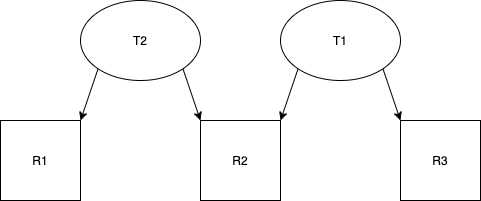
\includegraphics[scale=0.5]{COMS352HW6Q5}\\
This diagram shows that there is no way to have a cycle which,
means that this system is deadlock free.
\section*{Question 6}
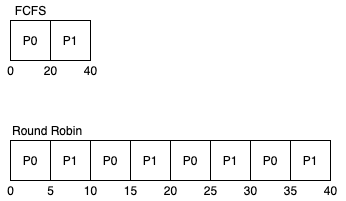
\includegraphics[scale=0.5]{COMS352HW6Q6}\\
The Round Robin algorithm could result in deadlock. If $P_0$ 
uses S and $P_1$ uses Q then they will both be waiting which 
means $P_0$ wont be able to use Q and $P_1$ can't use S. The 
FCFS algorithm is sequential however, which results in no deadlock.
\section*{Question 7}
\begin{itemize}
    \item \textbf{a.}\\
        No deadlock because no cycle is present. A possible execution 
        plan could be:\\ 
        $T_2$ --$>$ $T_3$ --$>$ $T_1$
    \item \textbf{b.}
        This graph is deadlocked. The cycle is:\\ 
        $T_1$ --$>$ $R_3$ --$>$ $T_3$ --$>$ $R_1$ --$>$ $T_1$
    \item \textbf{c.}
        No deadlock because no cycle is present. A possible execution 
        plan could be:\\ 
        $T_3$ --$>$ $T_1$ --$>$ $T_2$
    \item \textbf{d.}
        This graph is deadlocked. The cycle is:\\
         $T_1$ --$>$ $R_2$ --$>$ $T_3$ --$>$ $R_1$ --$>$ $T_1$
    \item \textbf{e.}
        No deadlock because there is no hold and wait condition.
        A possivle execution plan could be: 
        $T_2$ --$>$ $T_1$ --$>$ $T_3$ --$>$ $T_4$
    \item \textbf{f.}
        No deadlock, R2, has 3 available instances and 
        3 connecting threads. A possible execution plan could 
        be: 
        $T_2$ --$>$ $T_4$ --$>$ $T_1$ --$>$ $T_3$
\end{itemize}
\end{document}